\documentclass[12pt,titlepage]{article}
\usepackage[margin=1.25in]{geometry}
\usepackage{graphicx,amsmath,minted}

%% Variables definition
\newcommand{\vSubject}{Advanced Database}
\newcommand{\vSubtitle}{Midterm Exam}
\newcommand{\vName}{Dicha Zelianivan Arkana}
\newcommand{\vNIM}{2241720002}
\newcommand{\vClass}{2i}
\newcommand{\vDepartment}{Information Technology}
\newcommand{\vStudyProgram}{D4 Informatics Engineering}

%% [START] Tikz related stuff
\usepackage{tikz}
\usetikzlibrary{svg.path,calc,shapes.geometric,shapes.misc}
\tikzstyle{terminator} = [rectangle, draw, text centered, rounded corners = 1em, minimum height=2em]
\tikzstyle{preparation} = [chamfered rectangle, chamfered rectangle sep=0.75em, draw, text centered, minimum height = 2em]
\tikzstyle{process} = [rectangle, draw, text centered, minimum height=2em]
\tikzstyle{decision} = [diamond, aspect=2, draw, text centered, minimum height=2em]
\tikzstyle{data}=[trapezium, draw, text centered, trapezium left angle=60, trapezium right angle=120, minimum height=2em]
\tikzstyle{connector} = [line width=0.25mm,->]
%% [END] Tikz related stuff

%% [START] Fancy header related stuff
\usepackage{fancyhdr}
\pagestyle{fancy}
\setlength{\headheight}{15pt} % compensate fancyhdr style
\fancyhead{}
\fancyfoot{}
\fancyfoot[L]{\thepage}
\fancyfoot[R]{\textit{\vSubject - \vSubtitle}}
\renewcommand{\footrulewidth}{0.4pt}% default is 0pt, overline for footer
%% [END] Fancy header related stuff

%% [START] Custom tabular command related stuff
\usepackage{tabularx}
\newcommand{\details}[2]{
    #1 & #2  \\
}
%% [END] Custom tabular command related stuff

%% [START] Figure related stuff
\newcommand{\image}[3][1]{
    \begin{figure}[h]
        \centering
        \includegraphics[#1]{#2}
        \caption{#3}
        \label{#3}
    \end{figure}
}
%% [END] Figure related stuff

\begin{document}
\begin{titlepage}
    \centering
    \vfill
    {\bfseries\LARGE
        \vSubject\\
        \vskip0.25cm
        \vSubtitle
    }
    \vfill
    
\includegraphics[width=6cm]{images/polinema-logo.png}
    \vfill
    {
        \textbf{Name}\\
        \vName\\
        \vskip0.5cm
        \textbf{NIM}\\
        \vNIM\\
        \vskip0.5cm
        \textbf{Class}\\
        \vClass\\
        \vskip0.5cm
        \textbf{Department}\\
        \vDepartment\\
        \vskip0.5cm
        \textbf{Study Program}\\
        \vStudyProgram
    }
\end{titlepage}

\section{Tugas}
\begin{enumerate}
    \item {
        Buatlah diagram relasi dari keempat table tersebut

        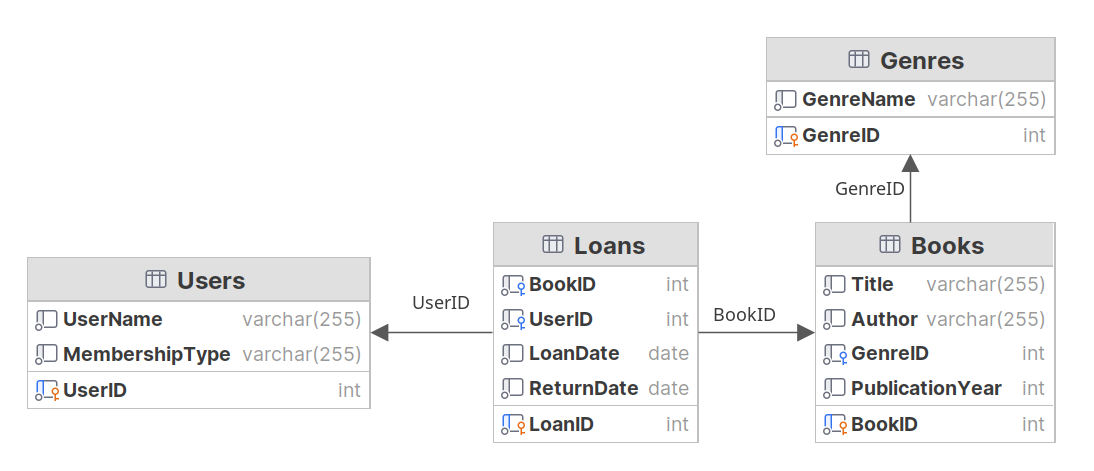
\includegraphics[width=.6\textwidth]{./images/diagram.png}
    }
    \item {
        Tampilkan semua isi semua tabel yang ada

        \begin{minted}[autogobble,fontsize=\small]{sql}
            SELECT * FROM Books;
        \end{minted}

        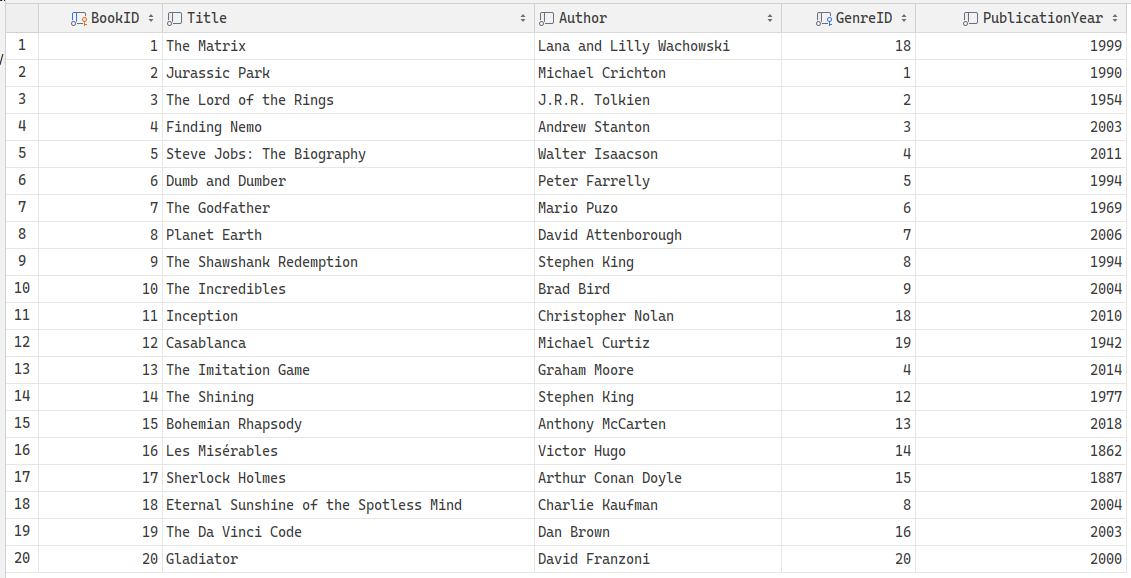
\includegraphics[width=.8\textwidth]{./images/books.png}

        \begin{minted}[autogobble,fontsize=\small]{sql}
            SELECT * FROM Genres;
        \end{minted}

        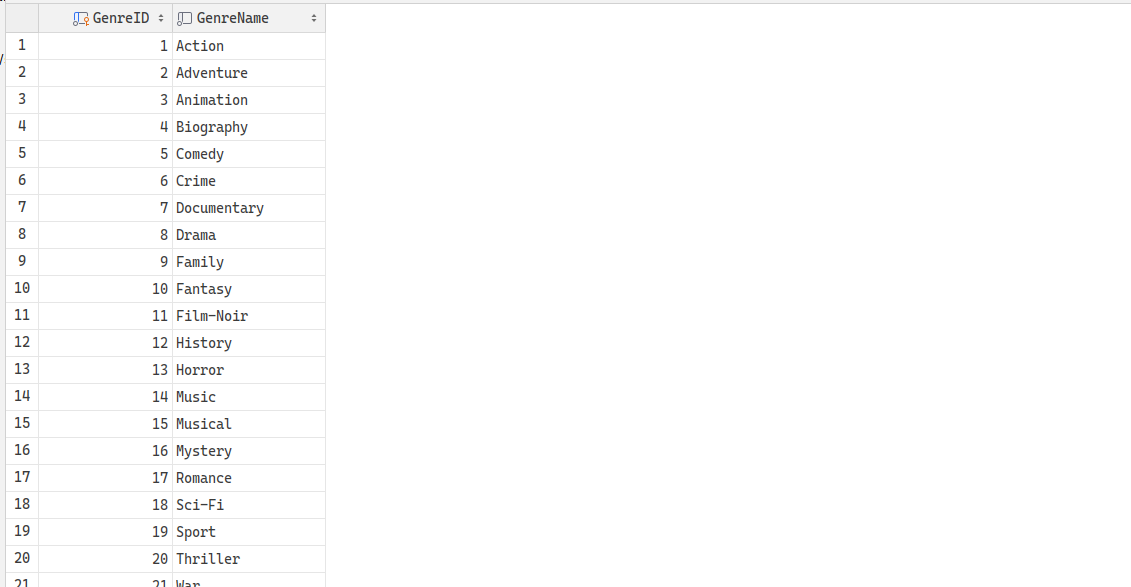
\includegraphics[width=.8\textwidth]{./images/genres.png}

        \pagebreak
        
        \begin{minted}[autogobble,fontsize=\small]{sql}
            SELECT * FROM Users;
        \end{minted}

        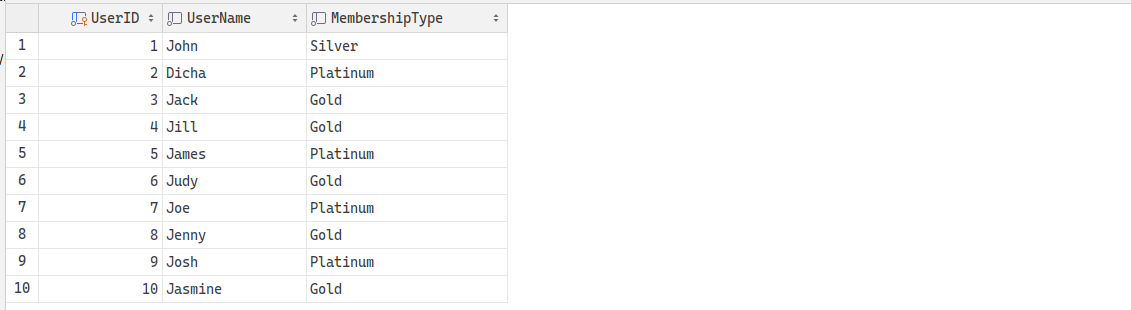
\includegraphics[width=.8\textwidth]{./images/users.png}

        \begin{minted}[autogobble,fontsize=\small]{sql}
            SELECT * FROM Loans;
        \end{minted}

        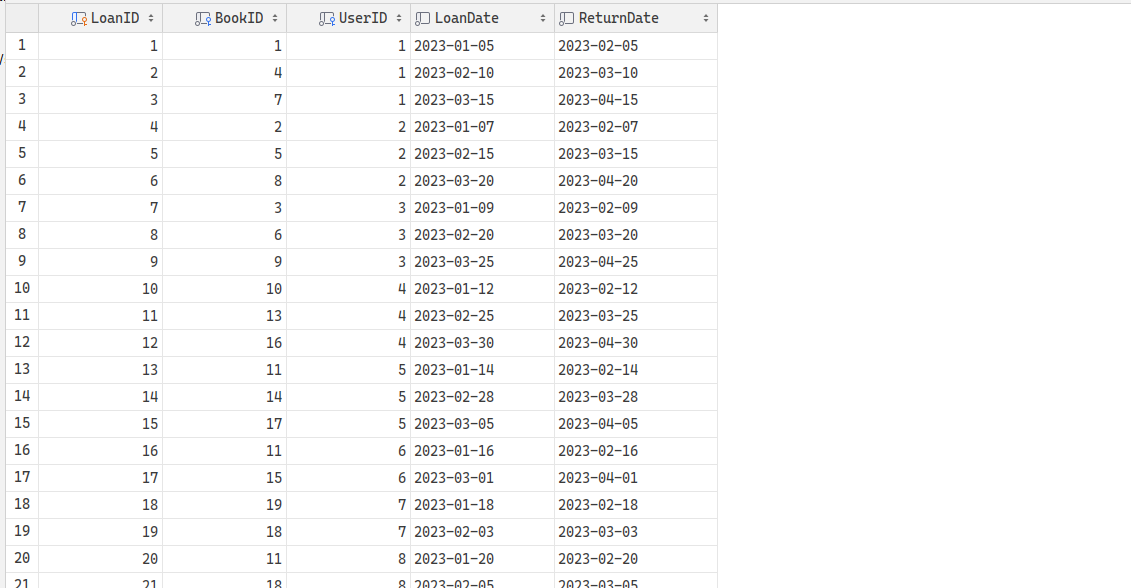
\includegraphics[width=.8\textwidth]{./images/loans.png}
    }
    \item {
        Tampilkan semua judul buku beserta nama penulisnya yang belum pernah dipinjam

        \begin{minted}[autogobble,fontsize=\small]{sql}
            SELECT Title, Author
            FROM Books
            WHERE BookID NOT IN (SELECT BookID FROM Loans);
        \end{minted}

        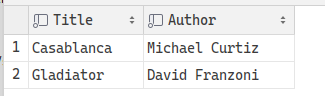
\includegraphics[width=.4\textwidth]{./images/3.png}
    }
    \pagebreak
    \item {
        Buatlah query untuk menemukan jumlah buku yang dipinjam per genre

        \begin{minted}[autogobble,fontsize=\small]{sql}
            SELECT
                GenreName,
                COUNT(Books.BookID) AS Jumlah
            FROM Books
                JOIN Genres ON Books.GenreID = Genres.GenreID
                JOIN Loans ON Books.BookID = Loans.BookID
            GROUP BY GenreName;
        \end{minted}

        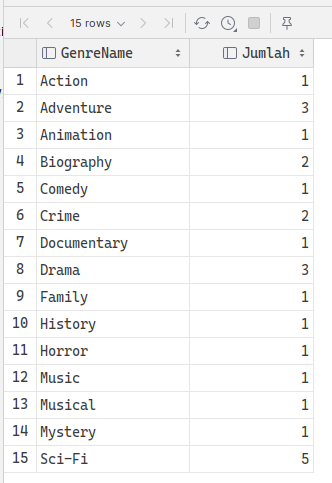
\includegraphics[width=.4\textwidth]{./images/4.png}
    }
    \pagebreak
    \item {
        Carilah jumlah total peminjaman per pengguna

        \begin{minted}[autogobble,fontsize=\small]{sql}
            SELECT
                UserName,
                COUNT(BookID) AS Jumlah
            FROM Loans
                JOIN Users ON Loans.UserID = Users.UserID
            GROUP BY UserName;
        \end{minted}

        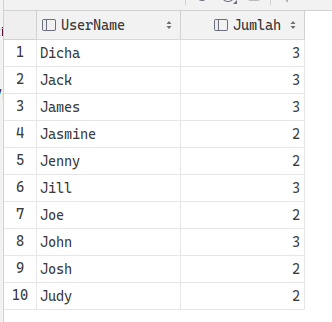
\includegraphics[width=.3\textwidth]{./images/5.png}
    }
    \item {
        Temukan buku yang paling sering dipinjam

        \begin{minted}[autogobble,fontsize=\small]{sql}
            SELECT 
                Title,
                COUNT(Loans.BookID) AS Jumlah
            FROM Loans JOIN Books ON Loans.BookID = Books.BookID
            GROUP BY Title
            ORDER BY Jumlah DESC
        \end{minted}

        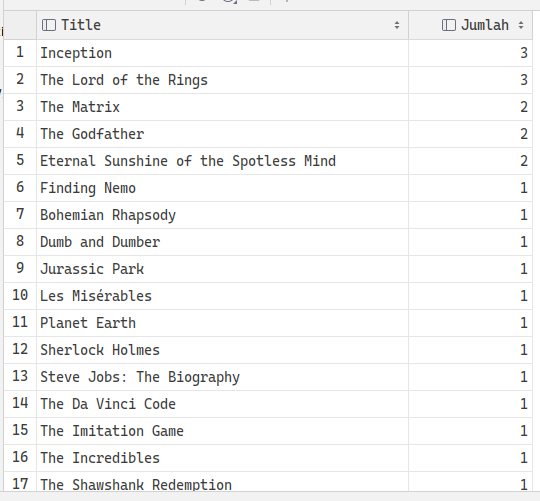
\includegraphics[width=.5\textwidth]{./images/6.png}
    }
    \pagebreak
    \item {
        Tentukan rata rata lama waktu peminjaman untuk setiap buku

        \begin{minted}[autogobble,fontsize=\small]{sql}
            WITH LoanDuration AS (
                SELECT BookID, DATEDIFF(day, LoanDate, ReturnDate) AS Duration
                FROM Loans
            )
            SELECT 
                Title,
                AVG(Duration) AS RataRata
            FROM LoanDuration
                JOIN Books ON LoanDuration.BookID = Books.BookID
            GROUP BY Title
            ORDER BY RataRata DESC;
        \end{minted}

        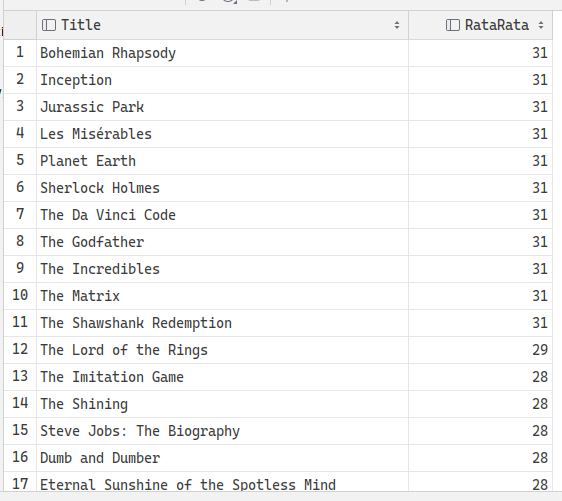
\includegraphics[width=.6\textwidth]{./images/7.png}
    }
    \pagebreak
    \item {
        Buatlah daftar pengguna dengan jumlah peminjaman diatas rata rata

        \begin{minted}[autogobble,fontsize=\small]{sql}
            WITH UserLoans AS (
                SELECT UserID, COUNT(BookID) AS Jumlah
                FROM Loans
                GROUP BY UserID
            )
            SELECT UserName, Jumlah
            FROM UserLoans
                JOIN Users ON UserLoans.UserID = Users.UserID
            WHERE Jumlah > (SELECT AVG(Jumlah) FROM UserLoans);
        \end{minted}

        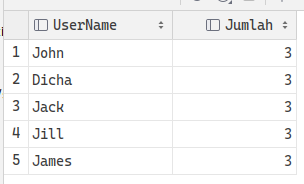
\includegraphics[width=.4\textwidth]{./images/8.png}
    }
    \item {
        Tampilkan histori peminjaman untuk buku dengan \texttt{BookID} tertentu

        \begin{minted}[autogobble,fontsize=\small]{sql}
            SELECT
                Title,
                UserName,
                LoanDate,
                ReturnDate
            FROM Loans
                JOIN Books ON Loans.BookID = Books.BookID
                JOIN Users ON Loans.UserID = Users.UserID
            WHERE Books.BookID = 1;
        \end{minted}

        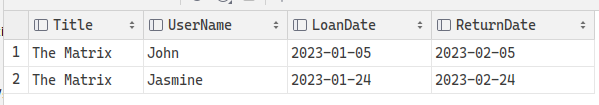
\includegraphics[width=.7\textwidth]{./images/9.png}
    }
    \pagebreak
    \item {
        Cari tahu siapa yang meminjam buku tertentu pada tanggal spesifik

        \begin{minted}[autogobble,fontsize=\small]{sql}
            SELECT
                UserName,
                Title,
                LoanDate,
                ReturnDate
            FROM Loans
                JOIN Users ON Loans.UserID = Users.UserID
                JOIN Books ON Loans.BookID = Books.BookID
            WHERE Books.BookID = 1
        \end{minted}

        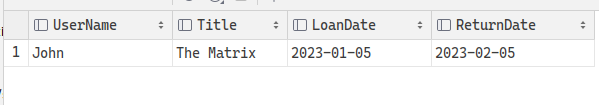
\includegraphics[width=.7\textwidth]{./images/10.png}
    }
    \item {
        Buatlah query untuk menampilkan buku yang paling lama dipinjam

        \begin{minted}[autogobble,fontsize=\small]{sql}
            WITH LoanDuration AS (
                SELECT
                    BookID,
                    DATEDIFF(day, LoanDate, ReturnDate) AS Duration
                FROM Loans
            )
            SELECT Title, Duration
            FROM LoanDuration
                JOIN Books ON LoanDuration.BookID = Books.BookID
            WHERE Duration = (SELECT MAX(Duration) FROM LoanDuration);
        \end{minted}

        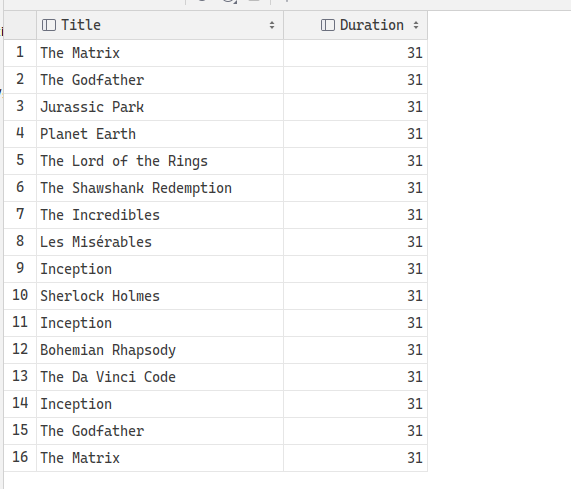
\includegraphics[width=.6\textwidth]{./images/11.png}
    }
    \item {
        Gunakan operasi pivoting untuk menampilkan jumlah buku yang dipinjam per bulan dalam tahun terakhir

        \begin{minted}[autogobble,fontsize=\small]{sql}
            SELECT
                Title,
                [1] AS Januari,
                [2] AS Februari,
                [3] AS Maret,
                [4] AS April,
                [5] AS Mei,
                [6] AS Juni,
                [7] AS Juli,
                [8] AS Agustus,
                [9] AS September,
                [10] AS Oktober,
                [11] AS November,
                [12] AS Desember
            FROM (
                SELECT
                    Title,
                    MONTH(LoanDate) AS Bulan
                FROM Loans
                    JOIN Books ON Loans.BookID = Books.BookID
                WHERE YEAR(LoanDate) = 2023
            ) AS SourceTable
            PIVOT (
                COUNT(Bulan)
                FOR Bulan IN ([1], [2], [3], [4],  [5],  [6],
                              [7], [8], [9], [10], [11], [12])
            ) AS PivotTable;
        \end{minted}

        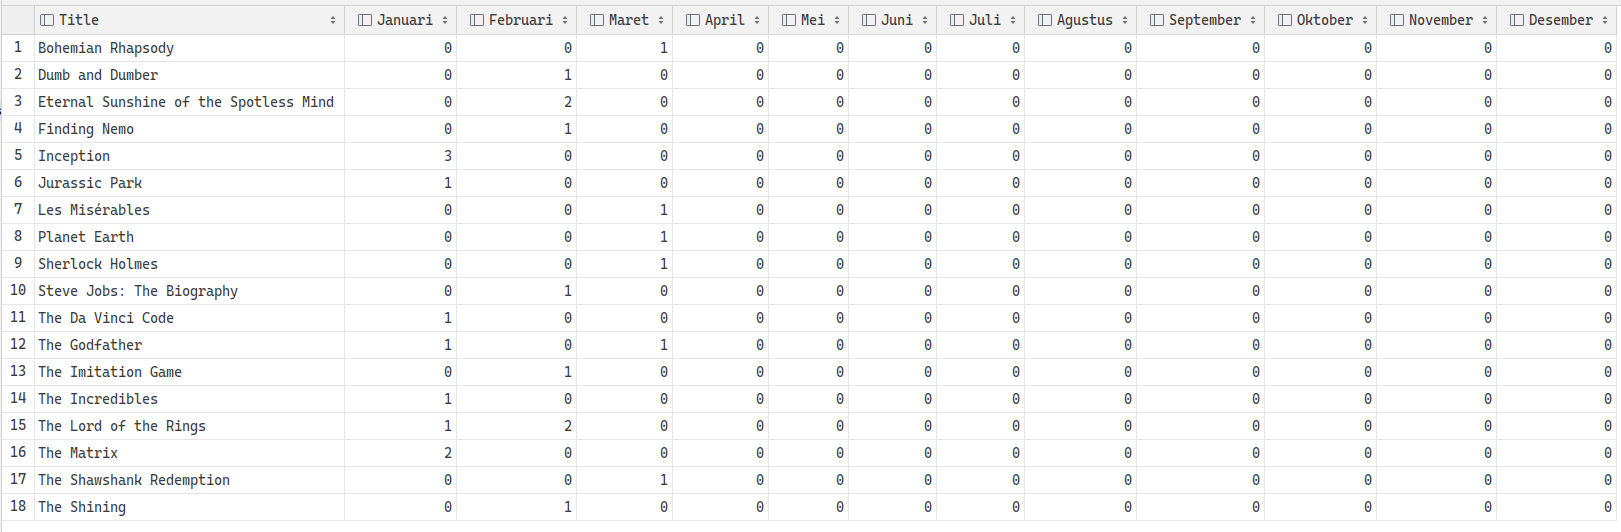
\includegraphics[width=.9\textwidth]{./images/12.png}
    }
\end{enumerate}

\end{document}

